\appendix
\addcontentsline{toc}{section}{Appendice}

\section{Resoconto attività di verifica}

\subsection{Verifica documentazione}
Per la verifica della documentazione si utilizza la tecnica del \glock{walkthrough} revisionando i documenti per intero e la tecnica di \glock{inspection} secondo i punti descritti nel documento \dext{norme di progetto v1.0.0}.

\subsubsection{Calcolo metriche gestione delle risorse}
Per verificare che i costi stabiliti rientrino in quanto preventivato si trovano a seguire dei grafici contenenti i risultati ottenuti:

	\paragraph{Budgeted cost of work scheduled}
		\begin{figure}[H]
			\centering
			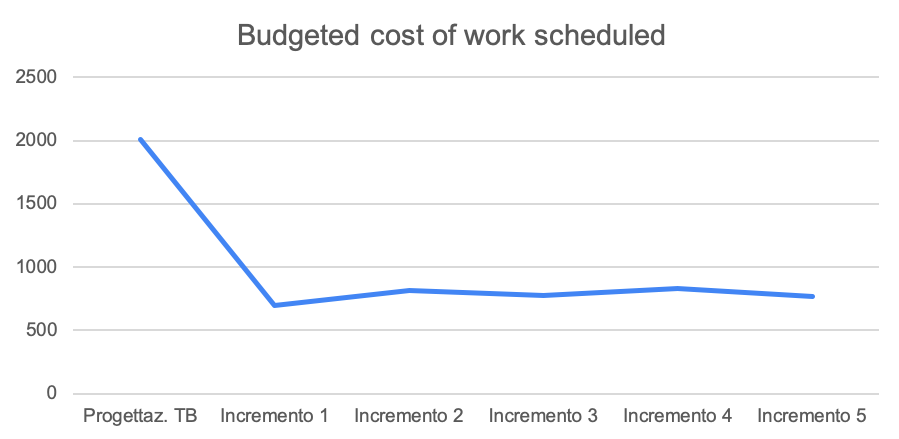
\includegraphics[width=0.8\linewidth]{./res/images/BCWS_1.png}
			\caption{Grafico }
			\label{fig:Grafico contenente il costo preventivato in Euro per fase}
		\end{figure}

	\paragraph{Actual cost of work performed}
		\begin{figure}[H]
			\centering
			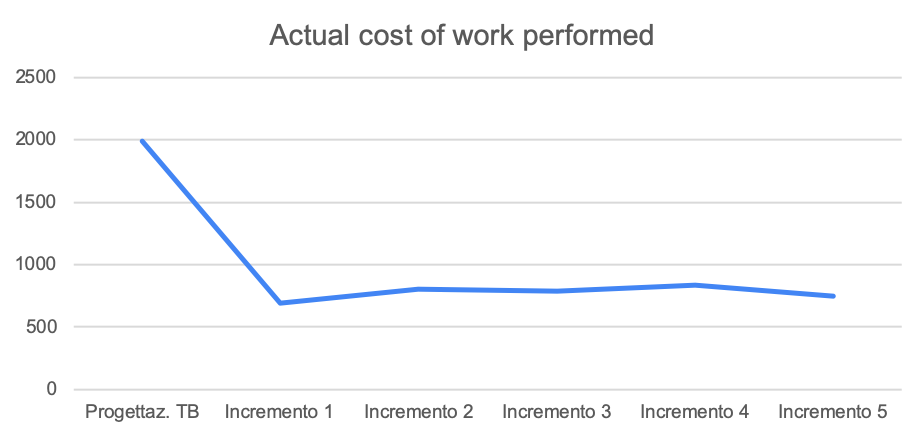
\includegraphics[width=0.8\linewidth]{./res/images/ACWP_1.png}
			\caption{Grafico }
			\label{fig:Grafico contenente il costo effettivo in Euro per fase}
		\end{figure}

	\paragraph{Budgeted cost of work performed}
		\begin{figure}[H]
			\centering
			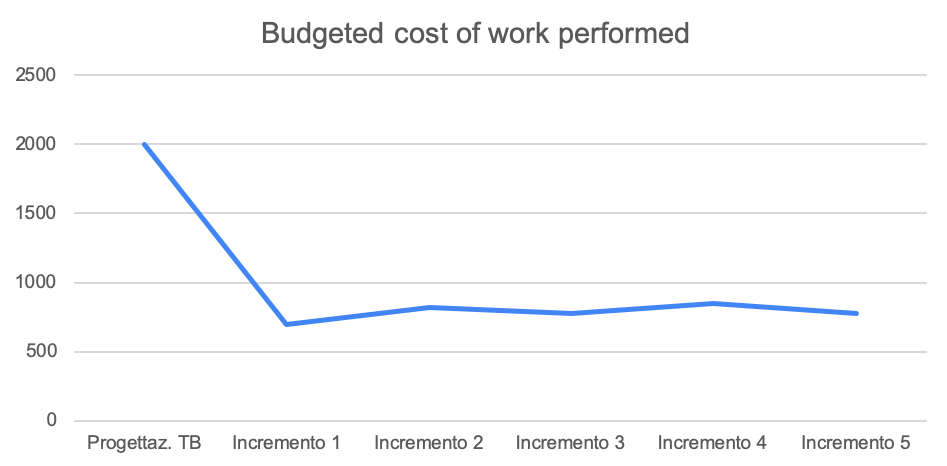
\includegraphics[width=0.8\linewidth]{./res/images/BCWP_1.png}
			\caption{Grafico }
			\label{fig:Grafico contenente il valore del prodotto in Euro per fase}
		\end{figure}

	\paragraph{Schedule variance}
		\begin{figure}[H]
			\centering
			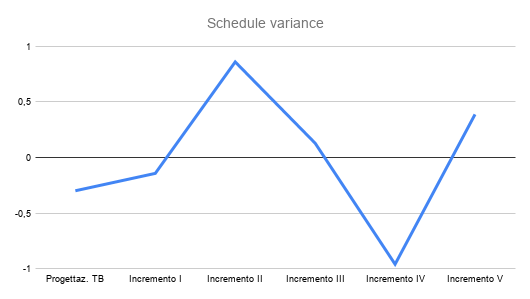
\includegraphics[width=0.8\linewidth]{./res/images/SV_1.png}
			\caption{Grafico }
			\label{fig:Grafico contenente la schedule variance per fase}
		\end{figure}

	\paragraph{Cost Variance}
		\begin{figure}[H]
			\centering
			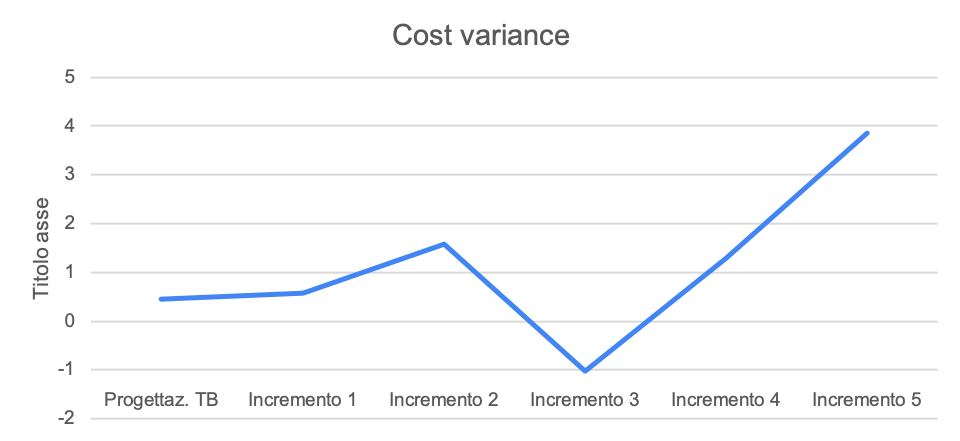
\includegraphics[width=0.8\linewidth]{./res/images/CV_1.png}
			\caption{Grafico }
			\label{fig:Grafico contenente la cost variance per fase}
		\end{figure}

\subsubsection{Calcolo metriche gestione dei rischi}
Per monitorare i rischi non preventivati riscontrati durante l'avanzamento del progetto si sono raccolte le misurazioni nel seguente grafico:
	
	\begin{figure}[H]
		\centering
		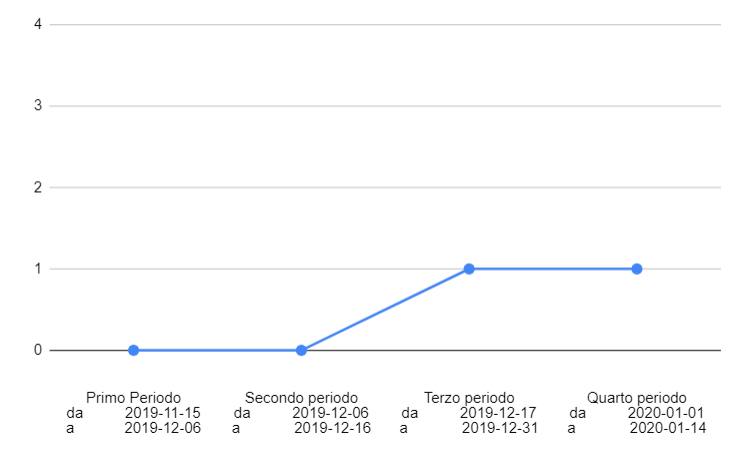
\includegraphics[width=0.8\linewidth]{./res/images/rischi.png}
		\caption{Grafico periodo/rischio nel periodo di analisi dei requisiti}
		\label{fig:Grafico periodo/rischio nel periodo di analisi dei requisiti}
	\end{figure}
	
	\begin{figure}[H]
			\centering
			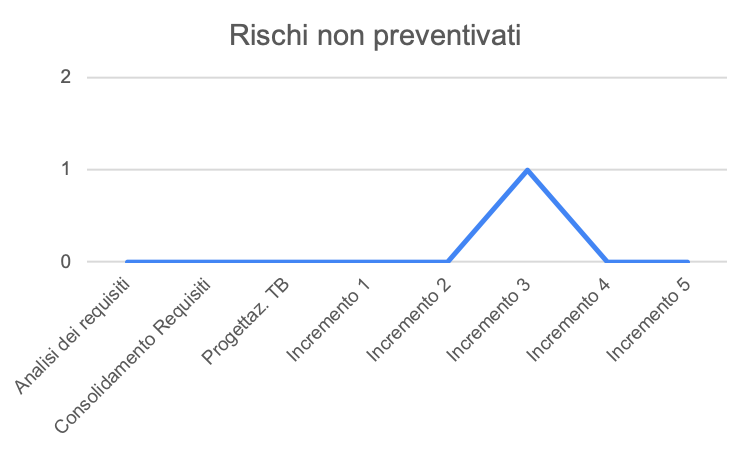
\includegraphics[width=0.8\linewidth]{./res/images/RischiNonPrevent_1.png}
			\caption{Grafico }
			\label{fig:Grafico i rischi non preventivati riscontrati in ogni fase}
		\end{figure}

\subsubsection{Calcolo leggibilità documenti}
Per verificare quanto sono leggibili i documenti redatti si utilizza \glock{l'indice di Gulpease}, di seguito il grafico contenente i risultati ottenuti durante il periodo di analisi dei requisiti:

\begin{figure}[H]
	\centering
	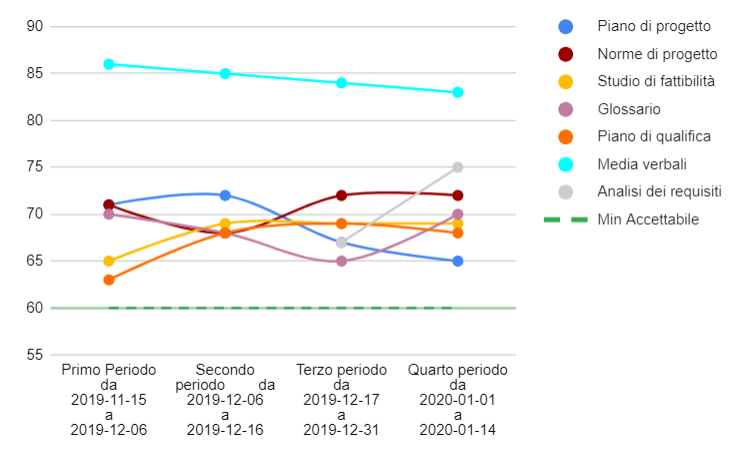
\includegraphics[width=0.8\linewidth]{./res/images/gulpease.png}
	\caption{Grafico periodo/indice di gulpease nel periodo di analisi dei requisiti}
	\label{fig:Grafico indice di gulpease periodo di analisi dei requisiti}
\end{figure}

\subsubsection{Calcolo ortografia documenti}
È stato effettuato un controllo di ortografia e di seguito vengono illustrati i risultati ottenuti durante il periodo di analisi dei requisiti:

\begin{center}
	\rowcolors{2}{lightest-grayest}{white}
	\begin{longtable}{|c|c|c|}
	\hline
	\rowcolor{lighter-grayer}
	\textbf{Documento} & \textbf{Errori ortografici} & \textbf{Accettabile} \\
	\hline
	\endfirsthead

	\hline
	Piano di Progetto & 0 & Sì \\
	\hline
	\hline
	Norme di Progetto &  0 & Sì \\
	\hline
	\hline
	Studio di fattibilità & 0 & Sì \\
	\hline
	\hline
	Glossario & 0 & Sì \\
	\hline
	\hline
	Piano di qualifica & 0 & Sì \\
	\hline
	\hline
	Media verbali & 0 & Sì \\
	\hline
	\hline
	Analisi dei requisiti & 0 & Sì \\
	\hline
	\caption{Tabella delle medie degli errori di ortografia durante il periodo di analisi dei requisiti}
	\end{longtable}
\end{center}

Di seguito il grafico riguardante gli errori rilevati durante il periodo di analisi dei requisiti:

\begin{figure}[H]
	\centering
	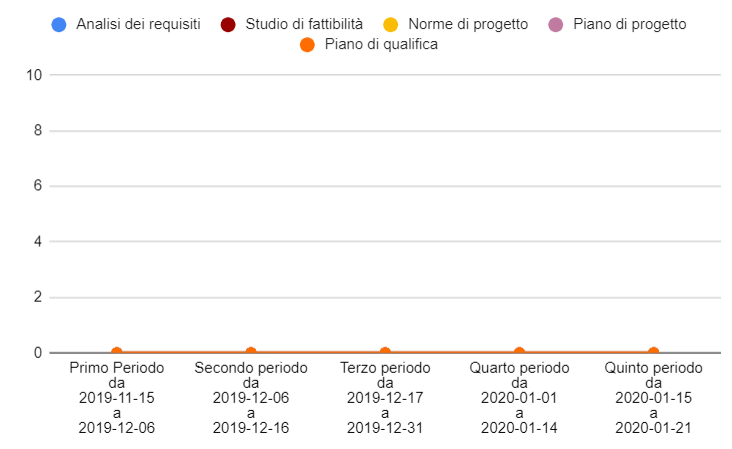
\includegraphics[width=0.8\linewidth]{./res/images/ortografia.png}
	\caption{Grafico periodo/errori ortografici nel periodo di analisi dei requisiti}
	\label{fig:Grafico errori ortografici durante il periodo di analisi dei requisiti}
\end{figure}
